\chapter{ACCOUNTING AND FINANCIAL STATEMENTS}
\begin{chapquote}{Unknown}
``Lotteries are simply “a tax on people bad at math”''
\end{chapquote}

\section{Cash versus accrual accounting}
Cash accounting is when you get cash from a customer and you count that as revenue for the current month. And any time you have to spend cash, you count that as an expense, again for the current month. This is what most small businesses do, while most slightly more sophisticated businesses would use accrual-based accounting, because that matches up the actual expenses and the revenue a little bit better in each period. 
The whole idea with accrual accounting is to match your revenues and expenses to when you actually perform the service. So it actually captures business activity, as opposed to just capturing when cash changes hands. Figure \ref{fig:cashVSaccrual} sums up the two accounting systems.

\begin{figure}[h!]
\centering
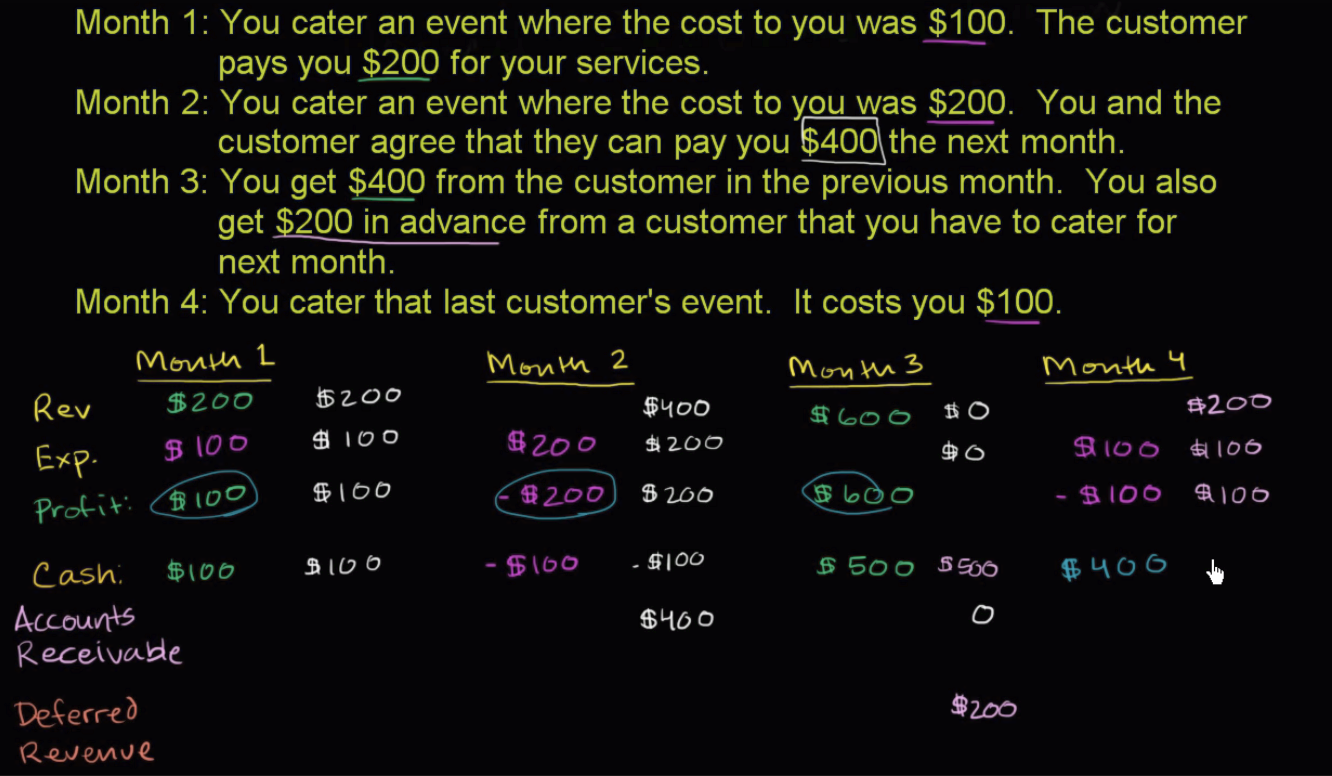
\includegraphics[width=0.8\textwidth]{images/cashVSaccrual.png}
\caption{Cash-based accounting (purple and green) vs accrual-based accounting (white). You should replace the hand pointer with \$400.}
\label{fig:cashVSaccrual}
\end{figure}

\section{Three core financial statements}

The income statement tells you what happens during a time period, while balance sheets are snapshots in time where you can see the cash (positive or negative, in which case would be debt to the bank for example), accounts receivable (money that you'll get in the future), deferred revenues (money that you have already received but you'll use in the future) and the resulting equity. The equity of a month corresponds also to the sum of the equity of the previous month plus the income reported in the income statement.

To keep track of what happens at a cash level, we have the cash flow statement. As we see from Figure \ref{fig:cashVSaccrual} in the cash line, at the end of the first month we have +\$100 and at the end of month 2 we have -\$100 nevertheless during month 2 according to the accrual-based accounting we made a profit of \$200. This is because we have the accounts receivable of +\$400. In the cash flow statement, we start from the cash at the end of a month, month 1 for example, we sum the net income, we subtract the accounts receivable (because we still don't have the cash) and we sum the deferred revenues (because we have the cash already). The result is the cash we get at the next month, month 2 in this case.

The historical cost is the amount of money spent on some initial good to start a business (land, factory, machines), while the fair value is how much they are worth now in the market, independently of the historical cost.

\section{Depreciation and amortization}

Depreciation and amortization spread the cost of an asset on its whole lifespan. The difference is that the former is for tangible assets (e.g., machines) the latter is for intangible assets (e.g., licenses, I.P.). 
